\chapter{Descripción del campo Teotleco}
\label{chp:campo}


\section{Ubicación}
El Proyecto de Explotación Cactus sitio Grande \emph{PECSG} se ubica a $32~[Km]$ al suroeste de la ciudad de Villahermosa, Tabasco, en la porción norte del estado de Chiapas, y es administrado por el Activo de producción Macuspana-Muspac, perteneciente a la Subdirección de Producción Región Sur de PEP. El PECSG lo integran $29$ campos, entre los que más destacan por su producción de petróleo crudo y gas son Teotleco, Cactus, Sunuapa, Juspí, Chiapas-Copano y Giraldas. 

    \begin{figure}[h]
        \centering
        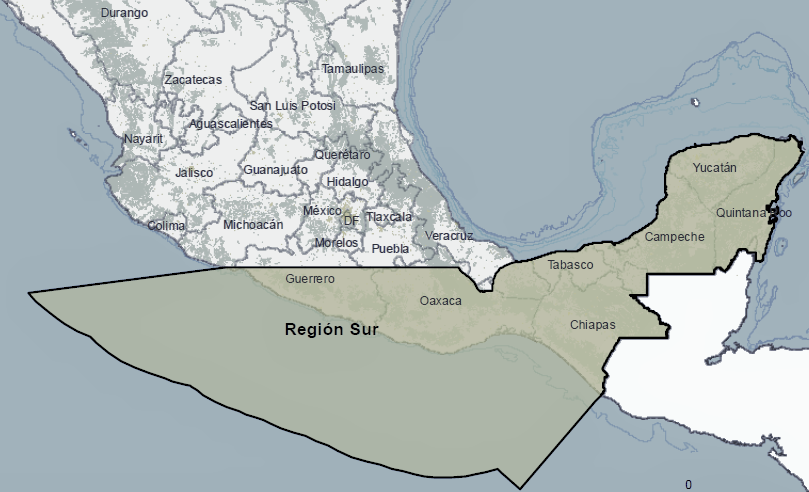
\includegraphics[width=0.9\textwidth]{Graphics/Region_Sur.png}
        \caption[Ubicación del Campo]{Cobertura geográfica de la región sur de PEP. Su extensión comprende los estados de Guerrero, Oaxaca, Veracruz, Tabasco, Campeche, Chiapas, Yucatán y Quintana Roo (Adaptado de \cite{PEMEX:2017})}
        \label{fig:PEPsur}
    \end{figure}


\section{Características de la roca}

El campo Teotleco se caracteriza por ser un yacimiento naturalmente fracturado de calizas y dolomías, con limitada continuidad de formaciones productoras debido a la falta de comunicación horizontal. Las formaciones productoras se encuentran a una profundidad de $5600~[m]$ en el Cretácico Superior y Cretácico Medio con un espesor neto de $70-100~[m]$, una porosidad de $5\%$ y una permeabilidad de entre $22-50~[mD]$. Teotleco al igual que otros campos del PECSG se ubican en cuencas asociadas con tectónicas salinas (\cite{PEMEX2012}).

\section{Características del Fluido}
EL tipo de fluido producido es un aceite volátil de alto encogimiento, con una gravedad API de $42~[\degree API]$ y con una relación gas-aceite de $520~[m^{3}/m^{3}] $ que se encuentra a una presión de $498~[Kg/cm^2]$ y $153~\celsius$ de temperatura a condiciones de yacimiento. El campo Teotleco tiene presencia de altos flujos fraccionales de agua y con tendencia a la deposición de inorgánicos.

El agua producida tiene una salinidad superior a $300~000~ppm STD$ con altos contenidos de Calcio($Ca^{+2}$) y Magnesio ($Mg^{+2}$). El desequilibrio termodinámico de estos iones así como la fuerza iónica del agua, conllevan a la depositación de sales.

\section{Producción}
Durante el $2014$, en conjunto, el PECSG con $164$ pozos produjeron $18404.7$ Mbpd de petróleo crudo y $95,242,955.2$ Mpcd de gas, el $65.5\%$ y $63.2\%$ de la producción total del activo de producción Macuspana-Muspac.
El campo Teotleco, por su parte, con $14$ pozos produjo $4,332.6 $ Mbpd y $18,136,131.3$ Mpcd lo que representó el $23.5\%$ y el $19\%$ de la producción total del activo (\cite{ASF2014}).


Debido a la alta canalización y por la colindancia de domos salinos la producción de agua congénita ha alcanzado un flujo fraccional en algunos pozos de hasta $80\%$, que junto con el taponamiento de las tuberías de producción, ha mermado la producción de aceite, incrementando los costos operativos y de mantenimiento para la intervención de pozos: limpieza y remoción de incrustaciones (\cite{CMP2017}).  

% LA INFORMACIÓN ESTA EN LA SIGUIENTE REFERENCIA, TE ENVIO EL ARCHIVO FUENTE.

% Martínez Ramírez I.E. 2012. Criticidad y solución para el desarrollo y administración del campo Teotleco. Activo de Producción Macuspana MUSPAC. Presentado en las Jornadas Técnicas AIPM, en Villahermosa Tabasco, Noviembre 09.